%\documentclass[landscape,a0paper,fontscale=0.285]{baposter} % a0 is 841mm x 1189mm
\documentclass[landscape,archE,fontscale=0.285]{baposter} % archE is 36in x 48in

% Define colors from UT web page
\selectcolormodel{RGB}
%\definecolor{utburntorange}{cmyk}{0,0.2549,0.3922,0.03529}
\definecolor{burntorange}{RGB}{191,87,0}
\definecolor{rightfooterorange}{RGB}{248,151,31}
\definecolor{pms432}{RGB}{51,63,72}
\definecolor{pms7469}{RGB}{0,95,134}
\definecolor{pms7572}{RGB}{214,210,196}
\definecolor{pms7543}{RGB}{156,173,183}


\usepackage{graphicx} % Required for including images
\graphicspath{{../fig}}

\usepackage{graphbox}
\usepackage{overpic}
\usepackage[caption=false]{subfig}

\usepackage{hyperref}
\hypersetup{
  colorlinks=true,
  urlcolor=pms432,
  pdftitle={Solving the Boltzmann transport equation for electron kinetics},
}

\usepackage{listings}
\lstset{numbers=left,
  basicstyle=\tiny\ttfamily,
  keywordstyle=\color{blue},
  breaklines=true,
  showtabs=false,
  showstringspaces=false,
  xleftmargin=2.5em,
}

\usepackage{amsmath} % For typesetting math
\usepackage{amssymb} % Adds new symbols to be used in math mode

\usepackage{booktabs} % Top and bottom rules for tables
\usepackage{enumitem} % Used to reduce itemize/enumerate spacing
\usepackage{palatino} % Use the Palatino font
\usepackage[font=small,labelfont=bf]{caption} % Required for specifying captions to tables and figures

\usepackage{multicol} % Required for multiple columns
\setlength{\columnsep}{1.5em} % Slightly increase the space between columns
\setlength{\columnseprule}{0mm} % No horizontal rule between columns

\usepackage{tikz} % Required for flow chart
\usetikzlibrary{shapes,arrows} % Tikz libraries required for the flow chart in the template

\newcommand{\compresslist}{ % Define a command to reduce spacing within itemize/enumerate environments, this is used right after \begin{itemize} or \begin{enumerate}
\setlength{\itemsep}{1pt}
\setlength{\parskip}{0pt}
\setlength{\parsep}{0pt}
}
\newcommand{\overbar}[1]{\mkern 1.5mu\overline{\mkern-1.5mu#1\mkern-1.5mu}\mkern 1.5mu}
\newcommand{\pp}[2]{\frac{\partial #1}{\partial #2}}
\newcommand{\dd}[2]{\frac{d #1}{d #2}}
\newcommand{\DD}[2]{\frac{D #1}{D #2}}
\newcommand{\mm}{\mathbf{minmod}}
\def\etal{{\it et al~}}
\newcommand{\be}{\begin{eqnarray}}
	\newcommand{\ee}{\end{eqnarray}}
\newcommand{\mbb}[1]{\mathbb{#1}} % math blackboard bold
\newcommand{\mcal}[1]{\mathcal{#1}} % math blackboard bold
\newcommand{\mbf}[1]{\mathbf{#1}} % math bold face (for vectors)
\newcommand{\sbf}[1]{\boldsymbol{#1}} % bold face for symbols
\newcommand{\jump}[1]{\llbracket #1 \rrbracket} % jump operator
\newcommand{\avg}[1]{\langle #1 \rangle} % average operator
\newcommand{\rarrow}{\rightarrow}
\newcommand{\Rarrow}{\Rightarrow}
\newcommand{\LRarrow}{\Leftrightarrow}
\newcommand{\vvvert}{|\kern-1pt|\kern-1pt|}
\newcommand{\enorm}[1]{\vvvert #1 \vvvert}
\newcommand{\nutil}{\tilde{\nu}}
\newcommand{\Var}{\mathrm{Var}}
\newcommand{\Cov}{\mathrm{Cov}}


\definecolor{MyDarkGreen}{rgb}{0,0.45,0.08}
\newcommand{\myred}[1]{{\color{red} #1}}
\newcommand{\myblue}[1]{{\color{blue} #1}}
\newcommand{\mygreen}[1]{{\color{MyDarkGreen} #1}}

\newcommand{\sa}{\nu_{\mathrm{sa}}}
\newcommand{\tep}{\tilde{\epsilon}}
\newcommand{\Ssd}{\mathcal{S}} % source term due to slow derivative
\newcommand{\ud}{\,\mathrm{d}}

\newcommand{\Mach}[1]{\ensuremath{\mbox{Ma}_{#1}}}
\newcommand{\Reynolds}{\ensuremath{\mathit{Re}}}
\newcommand{\DensityRat}{\ensuremath{\mathit{DR}}}
\newcommand{\BlowRat}{\ensuremath{\mbox{BR}}}
\newcommand{\VelRat}{\ensuremath{\mathit{VR}}}
\newcommand{\Tau}{\ensuremath{\mathrm{T}}}

\newcommand{\wall}     {\ensuremath{\mathrm{w}}}   % wall subindex
\newcommand{\awall}    {\ensuremath{\mathrm{aw}}}  % adiabatic wall subindex

\newcommand{\commentout}[1]{}

\newcommand{\vect}[1]{\boldsymbol{#1}}
\usepackage{mleftright}
\newcommand{\of}[1]{\mleft( #1 \mright)}
\newcommand{\vth}{v_{\textrm{th}}}
\newcommand{\reals}{\mathbb{R}}
\newcommand{\myint}{\int\limits}
\newcommand{\ddt}[1]{\partial_t #1}
\newcommand{\RR}{\mathbb{R}}
\newcommand{\vr}{v}
\newcommand{\diff}[1]{\, d#1}
\newcommand{\norm}[1]{\left\lVert#1\right\rVert}
%\newcommand{\vtheta}{\theta_{\vect{v}}}
%\newcommand{\vphi}{\varphi_{\vect{v}}}
%\newcommand{\vr}{v_{r}}
\newcommand{\vtheta}{{v_{\theta}}}
\newcommand{\vphi}{v_{\varphi}}
\newcommand{\vomega}{v_{\omega}}
\newcommand{\vrunit}{\hat{\vect{v}}_{r}}
\newcommand{\vthetaunit}{\hat{\vect{v}}_{\theta}}
\newcommand{\vphiunit}{\hat{\vect{v}}_{\varphi}}
\DeclareMathOperator{\variance}{Var}


\begin{document}

\begin{poster}
{
columns=4, % number of columns (change to suite your needs)
headerborder=closed, % Adds a border around the header of content boxes
colspacing=1em, % Column spacing
bgColorOne=white, % Background color for the gradient on the left side of the poster
bgColorTwo=white, % Background color for the gradient on the right side of the poster
borderColor=burntorange, % Border color
headershade=plain,
headerColorOne=burntorange, % Background color for the header in the content boxes (left side)
headerColorTwo=burntorange, %burntorange, % Background color for the header in the content boxes (right side)
headerFontColor=white, % Text color for the header text in the content boxes
boxColorOne=white, % Background color of the content boxes
textborder=roundedleft, % Format of the border around content boxes, can be: none, bars, coils, triangles, rectangle, rounded, roundedsmall, roundedright or faded
eyecatcher=false, %true, % Set to false for ignoring the left logo in the title and move the title left
headerheight=0.09\textheight, % Height of the header
headershape=roundedright, % Specify the rounded corner in the content box headers, can be: rectangle, small-rounded, roundedright, roundedleft or rounded
headerfont=\Large\bf\textsc, % Large, bold and sans serif font in the headers of content boxes
%textfont={\setlength{\parindent}{1.5em}}, % Uncomment for paragraph indentation
linewidth=2pt % Width of the border lines around content boxes
}
%----------------------------------------------------------------------------------------
% TITLE SECTION (spans whole width)
%----------------------------------------------------------------------------------------
%
{}
{\bf\textsc{Solving the Boltzmann transport equation for electron kinetics}\vspace{0.01em}} % Poster title
{\textsc{\small \textbf{Milinda Fernando}, George Biros, James Almgren-Bell, Todd Oliver, Laxminarayan Raja, Philip Varghese, Robert Moser  \hspace{12pt} \\The University of Texas at Austin}} % Author names and institution
{\includegraphics[align=c,height=0.09\textheight]{where_we_fit.png}% just figure (must edit fig to add highlight box)
%\raisebox{-0.5\height}{\begin{overpic}[height=0.09\textheight]{pecos_roadmap_tst_1.5.pdf} % figure + highlight box
%    \put(-1,8){\filldraw [semithick, fill=rightfooterorange, fill opacity=0.1, draw=gray, rounded corners] (1.9,1.2) rectangle +(1.15,0.7);}
%\end{overpic}}%
\hspace{12pt} \includegraphics[align=c,height=3em]{psaap3-logo.png}%
\hspace{12pt} \includegraphics[align=c,height=3em]{oden_pecos_2020_wordmark.png}%
}


\headerbox{Introduction}{name=introduction,column=0,row=0}{
\begin{itemize}
	\item Electron distribution function $f\of{t,\vect{v}, \vect{x}}$ defines the transport and kinetic properties.
	\item Evolution of $f$ is described by the Boltzmann equation.
	\begin{align*}
		\footnotesize
		\partial_t f + \vect{v}\cdot \nabla_{\vect{x}} f  - \frac{\vect{E} q}{m} \cdot \nabla_{\vect{v }}f = C_{en}(f) + C_{ee}(f,f)
	\end{align*}
	\item Electric field $\vect{E}$ causes acceleration in the v-space, while the collision operators $C_{en}$ and $C_{ee}$ describes the underlying collisions. 
\end{itemize}
}

\headerbox{Objectives}{name=objectives, below=introduction, column=0,row=1}{
\begin{itemize}
	\item \textbf{\textcolor{orange}{Main}}: Fast Boltzmann solver to determine electron kinetics properties $\rightarrow$ accurate low-temperature plasma simulations. 
	\item \textbf{\textcolor{orange}{Representation}}: Identify robust, yet low cost efficient representation of the distribution function $f(t, \vect{v}, \vect{x})$.
	\item \textbf{\textcolor{orange}{Challenges}}: Dimensionality of the problem (6 + 1 dimensions), numerical + HPC challenges.
\end{itemize}
\vspace{0.3em} % When there are two boxes, some whitespace may need to be added if the one on the right has more content
}

\headerbox{0D3V-BTE}{name=method_0D, below=objectives, above=bottom, column=0,row=2}{
	\begin{itemize}
		\item $f$ is approximated as isotropic + anisotropic correction terms.\\
			$
			\qquad 
			f(\vect{v},t) = \sum_{klm} f_{klm} \Phi_k\of{v} Y_{lm}\of{v_\theta, v_\phi}$
			$ \\
			\qquad 
			\text{ with }
			\phi_{pqs}\of{\vect{v}} = \underbrace{\Phi_p\of{v}}_{\text{radial basis}} \underbrace{Y_{qs}\of{v_\theta, v_\phi}}_{\tiny\text{sph. harm.}}$
		\item Weak formulation.\\
			$
			\displaystyle
			\quad
			\partial_t f - \frac{\vect{E} q}{m} \cdot \nabla_{\vect{v}}f = C(f)$
			$
			\Rightarrow
			\partial_t \myint_{R^3} f \phi\of{\vect{v}} \ud \vect{v} = \myint_{R^3} \of{C(f) + \of{\frac{\vect{E} q}{m} \cdot \nabla_{\vect{v}} f}} \phi\of{\vect{v}} \ud \vect{v} \forall \phi\of{\vect{v}}$	 	
		\item Currently implemented, 1). $C_{en}$: electron-heavy collisions, 2). $C_{ee}$: electron-electron Coulomb collisions
		\item $\hat{f} = \frac{f}{n_e}$ , $n_e = \int_{\vect{v}} f \diff{\vect{v}}$ with,\\
		$
		\displaystyle
		\quad
		\partial_t \hat{f} = (C+E)\hat{f} + n_e C_{ee}(\hat{f}, \hat{f}) -(u^T C_{en} \hat{f}) \hat{f} \\
		\text{ with } u^T \hat{f} =1
		$
		\begin{itemize}
			\item static $\vect{E}$-field : direct steady-state solutions
			\item oscillatory $\vect{E}$-field : cycle averaged transient solution
		\end{itemize}
		
	\end{itemize}
}

\headerbox{0D3V-Batched solver}{name=method_0D_B, above=method_0D, column=1,row=0}{
	\begin{itemize}
		\item \textbf{Application}: Launch 0D-BTE solves for each spatial point in fluid-approximation of plasma (see poster by Umberto Villa)
		\item Input : Heavy gas temperature $T_g(\vect{x})$, heavy and ion densities $n_0(\vect{x}), n_i(\vect{x})$, electric field $\vect{E}(\vect{x}, t)$
		\item Output : electron kinetics and reaction rates with 0D-BTE (steady-state, cycle averaged transient)
	\end{itemize}
	\vspace{-0.4in}
	\begin{center}
		\includegraphics[width=\columnwidth]{tps_0d_clusters.png}
		\captionof{figure}{Illustration of heavy temperature ($T_g$) based clustering of spatial points for underlying plasma simulation}
	\end{center}
	\vspace{-0.25in}
	\begin{itemize}
		\item Right-hand-side computation done by stacking BTE DoFs 
		\vspace{-0.25in}
		\begin{align*}
			\hspace{-0.25in}
			&\underbrace{C_{en}, C_{ee}, A_{v}}_{\text{pre-computed v-space operators}} \underbrace{\begin{bmatrix}
				\vdots & \vdots & \hdots &\vdots\\
				f_1    & f_2    & \hdots & f_{N_A} \\
				\vdots & \vdots & \hdots &\vdots
			\end{bmatrix}}_{\text{batched DoFs for cluster A}}
		\end{align*}
		\vspace{-0.25in}
		\item \textbf{Parla} for parallelization between clusters
	\end{itemize}
	
}

\headerbox{1D3V-BTE}{name=method_1D, below=method_0D_B, above=bottom, column=1,row=0}{
	\begin{center}
		\includegraphics[width=0.6\columnwidth]{glow1.png}
		\captionof{figure}{Glow discharge experiment setup}
	\end{center}
	{\footnotesize
	\begin{align*}
		&\partial_t f + v\cos\of{\vtheta} \partial_z f -\vect{E}\cdot\nabla_v f = C[f] \\
		&\textcolor{red!80}{f(\vect{v}, 0, t, \vtheta \leq \frac{\pi}{2})	= 0 \text{ and } f(\vect{v}, L, t, \vtheta > \frac{\pi}{2})	= 0}\\
		&\partial_t n_i + \partial_z \of{\mu_i n_i E\of{z,t} -D_i \partial_z n_i} = n_0 \gamma \myint_{\varepsilon}\myint_{\vect{\omega}} \varepsilon^{1/2} \sigma_i f d\vect{\omega} d\varepsilon \\
		& \vect{E} = \nabla \of{\Delta^{-1}\frac{e}{\epsilon_0} \of{n_i- n_e}} \text{ , } n_e = \myint_{\vect{v}} f\of{\vect{v}, z, t} \diff{\vect{v}}
	\end{align*} }%
	
	\begin{itemize}
		\item collocation method in $v_\theta$ and $x$ %  Use method of discrete ordinates in $\vtheta$, $f_{\vtheta_j} = f(v, \vtheta_j, z, t)$
		{\footnotesize
		\begin{align*}
			\partial_t f_{\vtheta_j} + v\cos\of{\vtheta_j} \partial_z f_{\vtheta_j} = P (C + E) P^{T}\begin{bmatrix}
				f_{\vtheta_0}\\
				\vdots\\
				f_{\vtheta_{N_\vtheta}}\\
			\end{bmatrix} %; %\\
			%j=1,..., N_{\vtheta} \nonumber
		\end{align*}}
		\vspace{-0.25in}
		\item Implicit time integration
		% \item Use B-splines + spherical basis representation of $f$ in the velocity-space for collision and v-space advection
		% \item Use finite difference method in $z$ direction
		% \item Use method of lines + with explicit time integrator in time
		% \item First order explicit operator splitting for evolving $n_i$ and $\vect{E}$ field equations
	\end{itemize}
}

\headerbox{0D3V-Results}{name=results_0D, column=2,row=0, above=bottom}{
	\textbullet~ Verification with Bolsig+\\
	\resizebox{0.9\columnwidth}{!}{
		\renewcommand{\arraystretch}{1.2}
		\begin{tabular}{|p{1cm}|p{1cm}|c|c|c|c|c|c|}
			\hline
			\multirow{2}{1cm}{\textbf{$E/n_0$ (Td)}} & \multirow{2}{1cm}{\boldmath$n_e/n_0$} & \multicolumn{6}{c|}{\textbf{relative error}}  \\
			% \hline
			% \textbf{Inactive Modes} & \textbf{Description}\\
			\cline{3-8}
			& & \textbf{energy} &\textbf{mobility} & \textbf{elastic} & \textbf{ionization} & {$\mathbf{f_0(\varepsilon)}$} & {$\mathbf{f_1(\varepsilon)}$}\\
			\hline
			1	  &  0 & 	3.40E-11 & 	3.30E-11	&  5.74E-11	&   -	     &   6.42E-08	&1.99E-07\\
			5	  &  0 & 	2.01E-10 & 	8.67E-10	&  2.69E-10	& 1.05E-08 &   1.08E-06	&3.77E-06\\
			20	&  0 &  3.64E-10 & 	1.55E-09	&  6.08E-10	& 1.58E-08 &   1.78E-07	&2.50E-06\\
			100 &  0 & 	3.62E-09 & 	5.10E-09	&  7.73E-09	& 1.20E-07 &   6.51E-07	&3.32E-06\\
			\hline                  
			1   &	$10^{-3}$ &	6.69E-07 &	7.21E-07 &	9.77E-07 &	4.77E-05 &	5.82E-07 &	1.28E-06\\
			5   &	$10^{-3}$ &	9.71E-08 &	1.08E-07 &	1.40E-07 &	1.59E-06 &	1.22E-07 &	2.00E-07\\
			20  &	$10^{-3}$ &	2.02E-09 &	4.09E-09 &	4.35E-09 &	7.94E-08 &	5.89E-07 &	5.23E-07\\
			100 &	$10^{-3}$ &	6.30E-09 &	4.08E-08 &	1.33E-09 &	2.21E-08 &	1.69E-05 &  1.82E-05\\
			\hline
			1   &	$10^{-2}$ &	9.57E-06 &	1.07E-05 &	1.39E-05 &	3.36E-04 &	8.29E-06 &	1.94E-05\\
			5   &	$10^{-2}$ &	4.04E-07 &	4.32E-07 &	5.87E-07 &	9.27E-06 &	3.65E-07 &	7.97E-07\\
			20  &	$10^{-2}$ &	6.97E-08 &	6.73E-08 &	8.67E-08 &	1.76E-06 &	1.70E-07 &	2.23E-07\\
			100 &	$10^{-2}$ &	4.04E-08 &	5.47E-08 &	4.67E-08 &	1.76E-07 &	3.05E-06 &	1.67E-06\\
			\hline
			1   &	$10^{-1}$ &	8.13E-05 &	1.07E-04 &	1.17E-04 &	1.69E-03 &	7.04E-05 &	1.94E-04\\
			5   &	$10^{-1}$ &	3.34E-06 &	4.23E-06 &	4.84E-06 &	5.24E-05 &	2.89E-06 &	7.61E-06\\
			20  &	$10^{-1}$ &	7.67E-07 &	8.58E-07 &	1.04E-06 &	1.07E-05 &	6.82E-07 &	1.62E-06\\
			100 &	$10^{-1}$ &	4.04E-08 &	1.79E-08 &	2.06E-08 &	6.06E-07 &	5.21E-07 &	7.14E-07\\
			\hline
		\end{tabular}
	}
	\begin{center}
		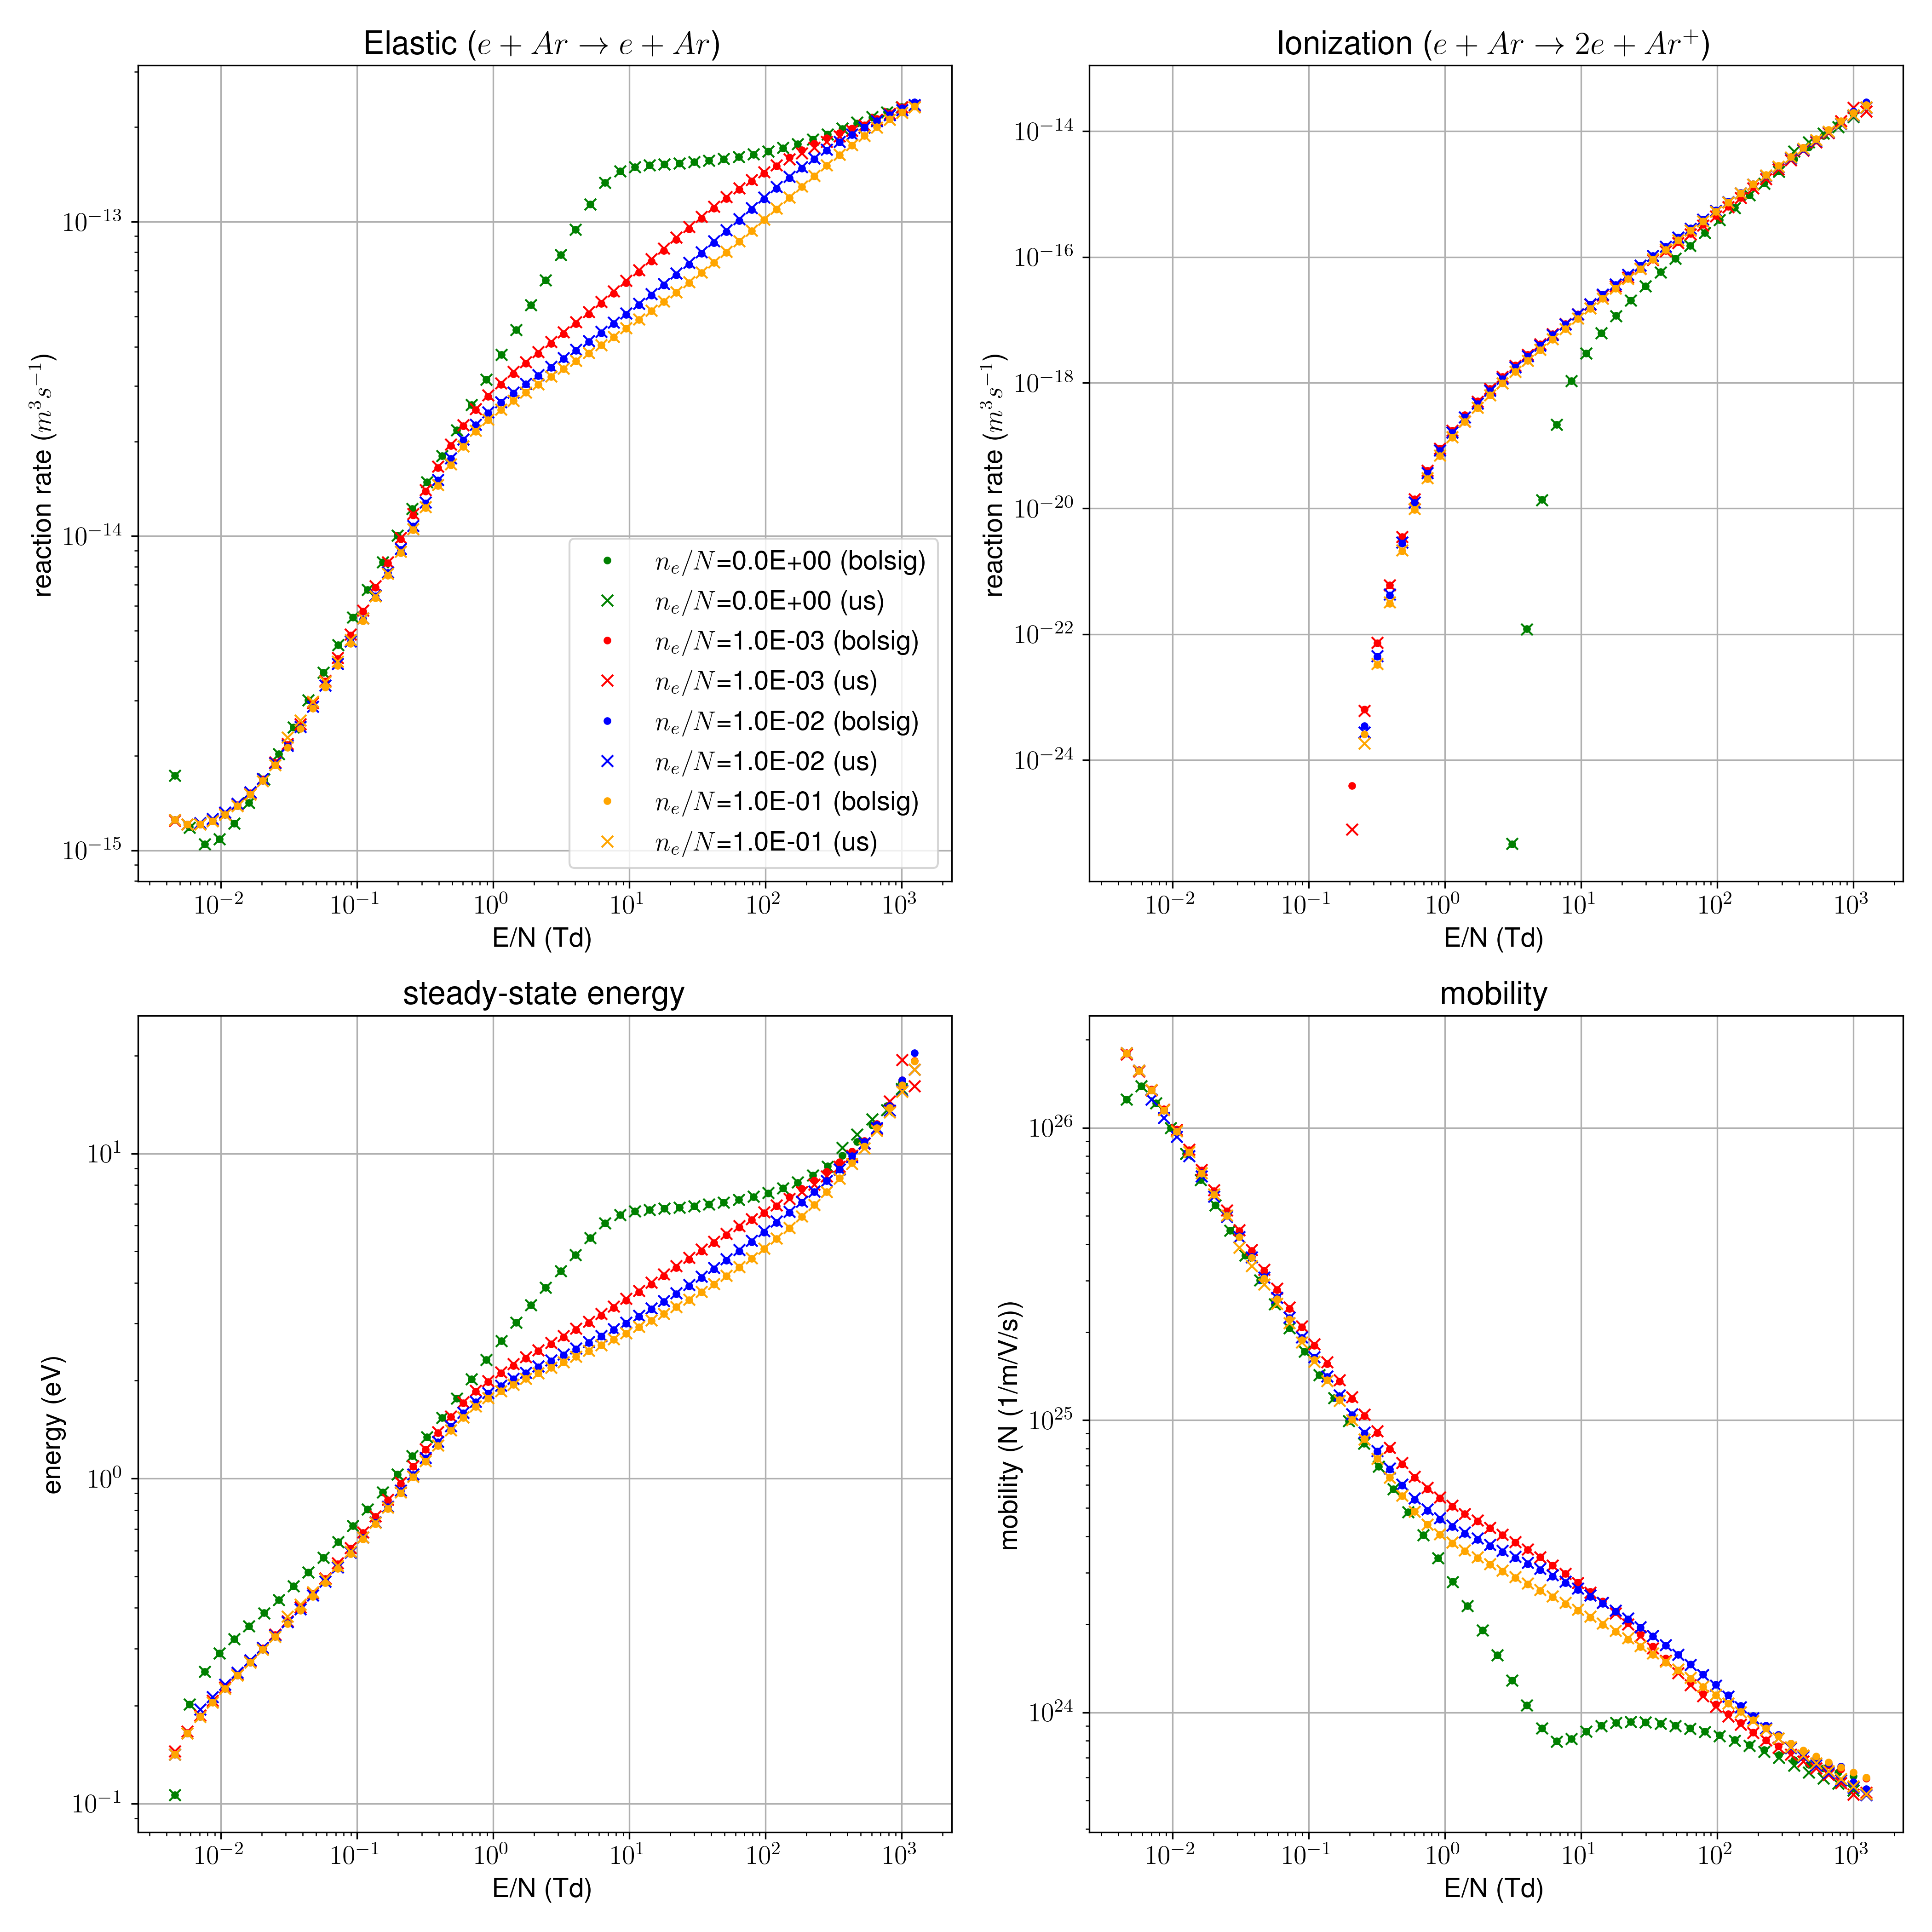
\includegraphics[width=0.8\columnwidth]{pde_vs_bolsig_with_coulomb_collision.png}
		\captionof{figure}{steady-state BTE comparison with Bolsig+}
	\end{center}
	\textbullet~ Beyond two-term approximation\\
	\begin{center}
		\includegraphics[width=0.48\columnwidth]{mf_verification_0.pdf}
		\includegraphics[width=0.48\columnwidth]{mf_verification_1.pdf}
		\includegraphics[width=0.48\columnwidth]{mf_verification_2.pdf}
		\includegraphics[width=0.48\columnwidth]{mf_verification_3.pdf}
		\captionof{figure}{multi-term comparison with PIC-DSMC code (see poster by James Almgren-Bell)}
	\end{center}
	
}

\headerbox{1D3V-Results}{name=results_1D, column=3,row=0}{
	\textbullet~ Low-voltage glow discharge with 1D-space Boltzmann
	\begin{center}
		\includegraphics[width=0.48\columnwidth]{1v_0.png}
		\includegraphics[width=0.50\columnwidth]{1v_1.png}
	\end{center}	
	\textbullet~ $P: \{\vtheta_{i}\} \mapsto \text{span}\{Y_{lm}\}$
	\begin{center}
		\includegraphics[width=0.85\columnwidth]{glow1d_adv_x.png}
		\captionof{figure}{Convergence of ordinates to spherical projection operator with increasing $lm$-modes}
	\end{center}
	\textbullet~ Advection in phase space ($\vect{x}, \vect{v}$)
	\begin{center}
		\includegraphics[width=0.85\columnwidth]{glow1d_adv_vx.png}
		\captionof{figure}{Convergence of advection in phase space with elastic electron-heavy collisions with static $\vect{E}$-field}
	\end{center}
}

\headerbox{Future work}{name=fw, column=3,row=0, above=bottom}{
	\begin{itemize}
		\item IMEX time integration for 1D3V-BTE glow discharge
		\item Analysis of Maxwellian rate coefficients and BTE approximations for glow discharge
		\item 1D3V, 2D3V BTE for the torch code
	\end{itemize}
}

%----------------------------------------------------------------------------------------
%	REFERENCES
%----------------------------------------------------------------------------------------

% \headerbox{References}{name=references,column=0,above=bottom}{

% \renewcommand{\section}[2]{\vskip 0.05em} % Get rid of the default "References" section title
% \nocite{*} % Insert publications even if they are not cited in the poster
% \small{ % Reduce the font size in this block
% \bibliographystyle{unsrt}
% \bibliography{sample} % Use sample.bib as the bibliography file
% }}

% %----------------------------------------------------------------------------------------
% %	FUTURE RESEARCH
% %----------------------------------------------------------------------------------------
%\headerbox{1D Glow Discharge}{name=glow_discharge,column=2,span=1,row=0}{
%\begin{center}
%	\includegraphics[width=0.7\textwidth]{eye-candy/glow/glow1.png}
%\end{center}
%\subsubsection*{Formulation}
%\footnotesize{
%\begin{align}
%	&\partial_t f + v\cos\of{\vtheta} \partial_z f -\vect{E}\cdot\nabla_v f = C[f] \\
%	&\textcolor{red!80}{f(\vect{v}, 0, t, \vtheta \leq \frac{\pi}{2})	= 0 \text{ and } f(\vect{v}, L, t, \vtheta > \frac{\pi}{2})	= 0}\\
%	&\partial_t n_i + \partial_z \of{\mu_i n_i E\of{z,t} -D_i \partial_z n_i} = N \gamma \myint_{\varepsilon}\myint_{\vect{\omega}} \varepsilon^{1/2} \sigma_i f d\vect{\omega} d\varepsilon \\
%	& \vect{E} = \nabla \of{\Delta^{-1}\frac{e}{\epsilon_0} \of{n_i- n_e}} \text{ , } n_e = \myint_{\vect{v}} f\of{\vect{v}, z, t} \diff{\vect{v}}
%\end{align}}
%\subsubsection*{Discretization}
%\begin{itemize}
%	\item Use method of discrete ordinates in $\vtheta$, $f_{\vtheta_j} = f(v, \vtheta_j, z, t)$
%	\footnote{
%	\begin{align}
%		\partial_t f_{\vtheta_j} + v\cos\of{\vtheta_j} \partial_z f_{\vtheta_j} = P_{\vtheta_j} (C + E) \begin{bmatrix}
%			f_{\vtheta_0}\\
%			\vdots\\
%			f_{\vtheta_{N_\vtheta}}\\
%		\end{bmatrix} ; \\
%		j=1,..., N_{\vtheta} \nonumber
%	\end{align}}
%	\item Use B-splines + spherical basis representation of $f$ in the velocity-space for collision and v-space advection
%	\item Use finite difference method in $z$ direction
%	\item Use method of lines + with explicit time integrator in time
%	\item First order explicit operator splitting for evolving $n_i$ and $\vect{E}$ field equations
%\end{itemize}
%}
%
%\headerbox{Future Work}{name=future_work,column=2,span=1,row=0,below=glow_discharge,above=bottom}{
%	\begin{itemize}
%	\item Add filtering in $\vtheta$ direction
%	\item Supports adaptive discrete ordinates in space
%	\item Integration with PyKokos and Parla
%	\item Revisit radial discretization
%	\begin{itemize}
%		\item DG or finite volume discretization
%	\end{itemize}
%	%\item Artificial diffusion in speed, for stabilization ?
%\end{itemize}
%}


%----------------------------------------------------------------------------------------
%	CONTACT INFORMATION
%----------------------------------------------------------------------------------------

%%% \headerbox{Contact Information}{name=contact,column=3,aligned=references,above=bottom}{ % This block is as tall as the references block
%%% \begin{description}\compresslist
%%% \item[Web] www.university.edu/smithlab
%%% \item[Email] john@smith.com
%%% \end{description}
%%% }

%----------------------------------------------------------------------------------------
%	CONCLUSION
%----------------------------------------------------------------------------------------

% \headerbox{Conclusions}{name=conclusions,column=0,span=4,below=method,above=bottom}{ % This block is as tall as the references block
% \begin{itemize}
%   \item We present an open-source framework to solve the velocity-space Boltzmann equation using Galerkin approach with tabulated cross-section data. Our framework goes beyond the traditional 2-term approximation for the distribution function. We provide efficient robust solvers for steady state and transient solutions. 
%   \item \textbf{Future Work} Add 1d3d solver for the plasma tourch simulations as an initial attempt
% \end{itemize}
% }

%----------------------------------------------------------------------------------------
%	RESULTS 1
%----------------------------------------------------------------------------------------

% \headerbox{Results}{name=results_0d3v,column=2,span=2,row=0,above=conclusions}{
% 	\begin{itemize}
% 		\item Self-convergence and comparison with Bolsig code (2-term expansion)
% 	\end{itemize}
% 	\begin{minipage}{0.4\textwidth}
% 	\resizebox{\textwidth}{!}{
% 		\renewcommand{\arraystretch}{1.2}
% 		\begin{tabular}{|p{1cm}|p{1cm}|c|c|c|c|c|c|}
% 			\hline
% 			\multirow{2}{1cm}{\textbf{E/N (Td)}} & \multirow{2}{1cm}{\boldmath$n_e/N$} & \multicolumn{3}{c|}{\textbf{rel. error vs. Bolsig}} & \multicolumn{3}{c|}{\textbf{rel. error (self convergence)}}\\
% 			% \hline
% 			% \textbf{Inactive Modes} & \textbf{Description}\\
% 			\cline{3-8}
% 			& & \textbf{elastic} & \textbf{ionization} & \textbf{mobility} & \textbf{elastic} & \textbf{ionization} & \textbf{mobility}\\
% 			%\hhline{~--}
% 			\hline
% 			1        & 0.0 & 7.11E-05 &    --	    & 4.10E-05	& 4.61E-12	&   --	    & 2.47E-12 \\
% 			5        & 0.0 & 4.12E-04 & 3.74E-04	& 2.92E-06	& 3.83E-07	& 3.84E-04	& 5.34E-07 \\
% 			20       & 0.0 & 5.76E-04 & 3.49E-03	& 2.98E-04	& 2.77E-04	& 9.74E-03	& 1.29E-03 \\
% 			100      & 0.0 & 1.35E-03 & 2.74E-03	& 4.85E-03	& 2.02E-03	& 4.11E-02	& 6.65E-04 \\
% 			\hline
% 			1        & $10^{-3}$ & 9.40E-03	& 4.40E-03	& 7.99E-03	& 8.61E-07	& 3.60E-05	& 6.40E-07 \\
% 			5        & $10^{-3}$ & 1.52E-02	& 4.12E-03	& 1.83E-04	& 1.66E-07	& 1.42E-06	& 1.31E-07 \\
% 			20       & $10^{-3}$ & 1.69E-02	& 1.46E-02	& 1.13E-02	& 6.93E-08	& 1.89E-07	& 6.68E-08 \\
% 			100      & $10^{-3}$ & 9.11E-03	& 1.87E-02	& 1.65E-02	& 1.53E-07	& 2.96E-07	& 2.50E-07 \\
% 			\hline
% 			1        & $10^{-2}$ & 4.88E-03	& 1.20E-02	& 9.94E-03	& 6.72E-06	& 1.77E-04	& 5.18E-06 \\
% 			5        & $10^{-2}$ & 7.85E-03	& 8.73E-03	& 9.56E-03	& 2.73E-07	& 4.87E-06	& 2.07E-07 \\
% 			20       & $10^{-2}$ & 1.13E-02	& 4.57E-03	& 6.19E-03	& 1.85E-08	& 4.32E-08	& 1.48E-08 \\
% 			100      & $10^{-2}$ & 1.19E-02	& 9.93E-03	& 7.76E-03	& 2.50E-08	& 3.24E-09	& 2.57E-08 \\
% 			\hline
% 			1        & $10^{-1}$ & 1.72E-03	& 8.17E-03	& 5.31E-03	& 4.39E-05	& 6.37E-04	& 4.01E-05 \\
% 			5        & $10^{-1}$ & 2.42E-03	& 7.80E-03	& 7.74E-03	& 5.49E-06	& 5.91E-05	& 4.79E-06 \\
% 			20       & $10^{-1}$ & 3.84E-03	& 7.97E-03	& 8.41E-03	& 5.46E-07	& 5.01E-06	& 4.59E-07 \\
% 			100      & $10^{-1}$ & 4.76E-03	& 9.80E-04	& 1.89E-03	& 3.97E-08	& 2.88E-07	& 3.35E-08 \\
% 			\hline
% 	\end{tabular}}
% 	\end{minipage}
% 	\begin{minipage}{0.6\textwidth}
% 		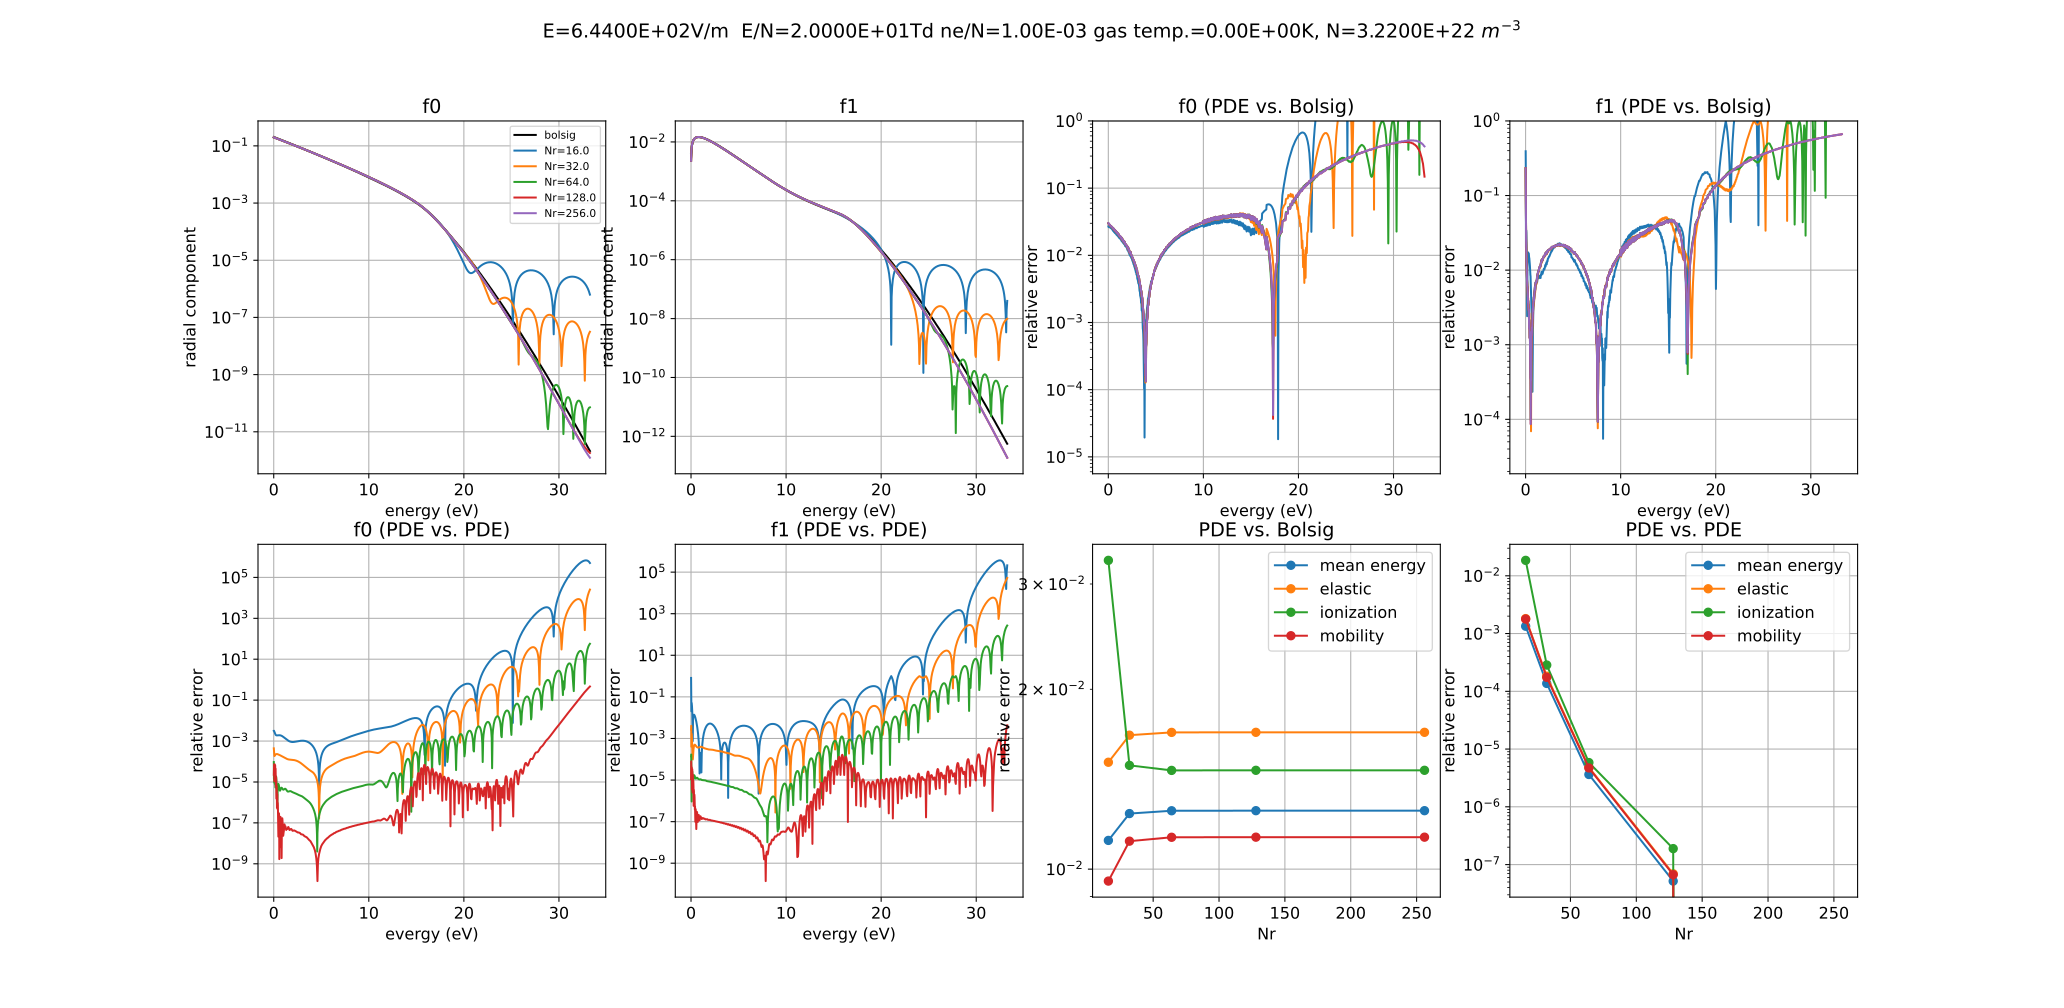
\includegraphics[width=\textwidth]{us_vs_bolsig_cg_g0_g2_E643.9999999999999_poly_bspline_sp_4_nr256_qpn_4_bscale1.0_sweeping_Nr_lmax_1_ion_deg_1.00E-03_Tg0.00E+00.png}
% 	\end{minipage}
% 	\begin{itemize}
% 		\item Effect on electron-electron collisions on the QoIs 
% 	\end{itemize}
% 	\begin{minipage}{0.99\textwidth}
% 		\centering
% 		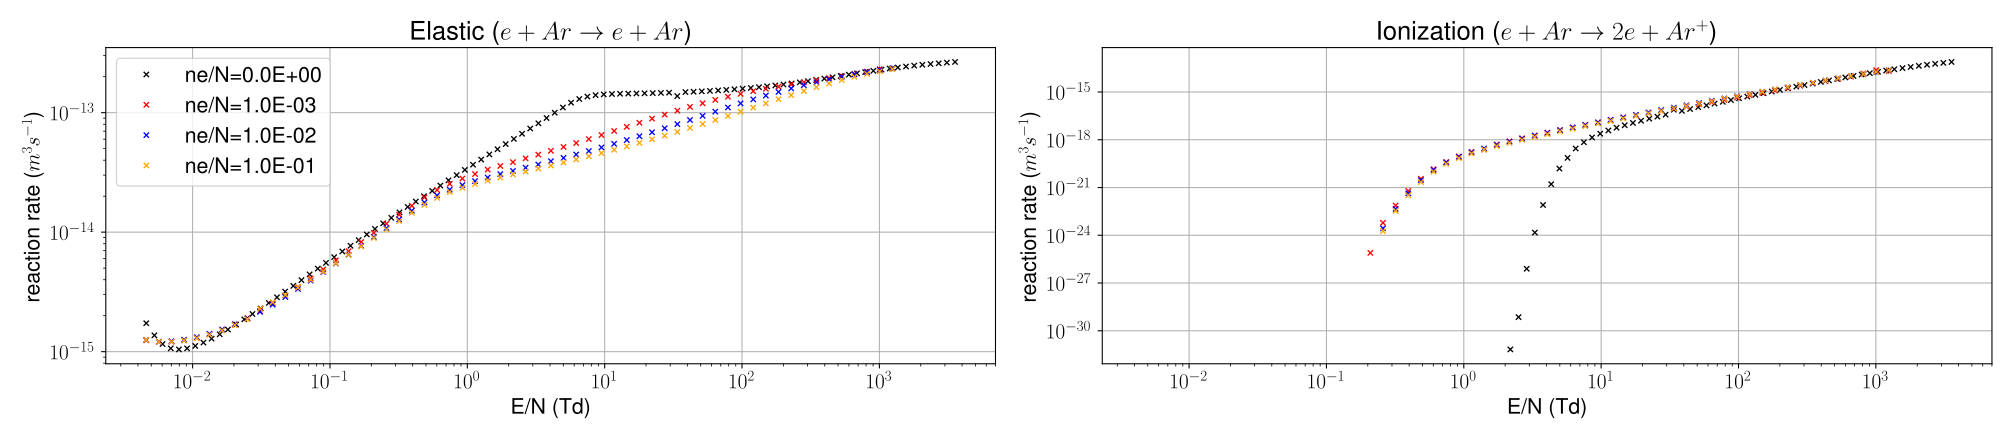
\includegraphics[width=\textwidth]{effect_of_cc.png}
% 	\end{minipage}
% 	\begin{center}
% 	\begin{minipage}{0.83\textwidth}

% 			\resizebox{\textwidth}{!}{
% 				\begin{tabular}{cc}
% 					$E/N=1Td,\ n_e/N = 0$ & $E/N=1Td,\ n_e/N = 1e-3$ \\ 
% 					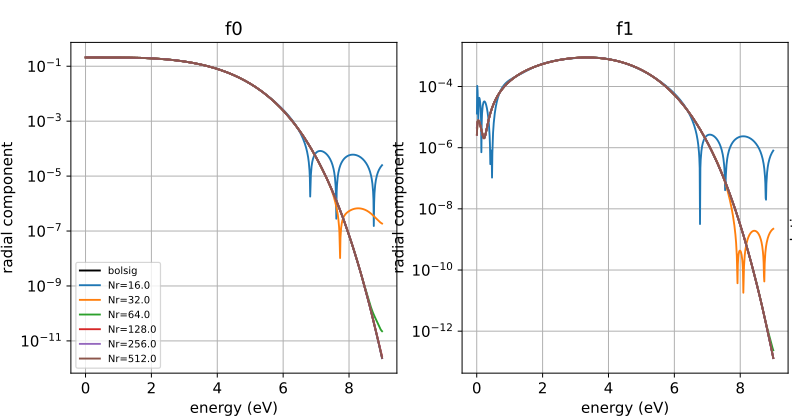
\includegraphics[width=0.48\textwidth]{1TD_ion_deg_0e0.png} & 	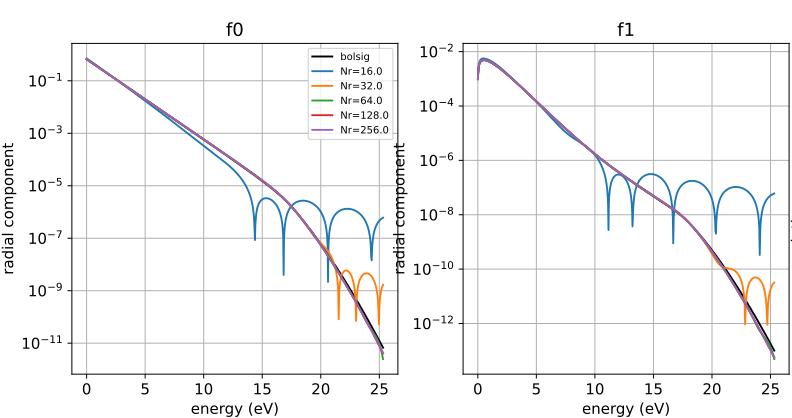
\includegraphics[width=0.48\textwidth]{1TD_ion_deg_1e-3.png}\\
% 					%		ne/N = 1e-2 & ne/N = 1e-1 \\ 
% 					%		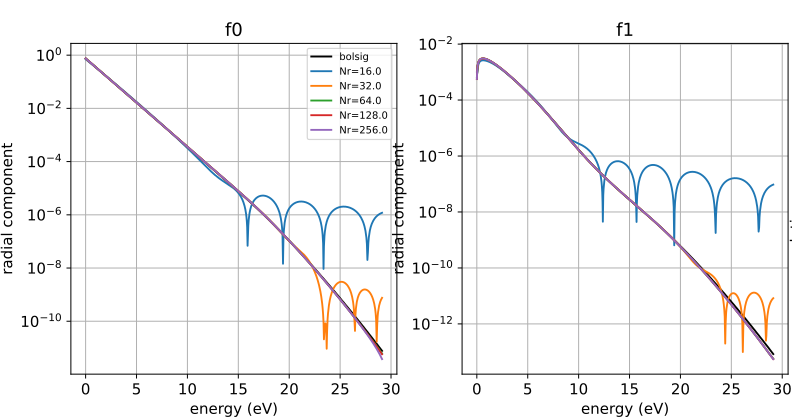
\includegraphics[width=0.48\textwidth]{1TD_ion_deg_1e-2.png} & 	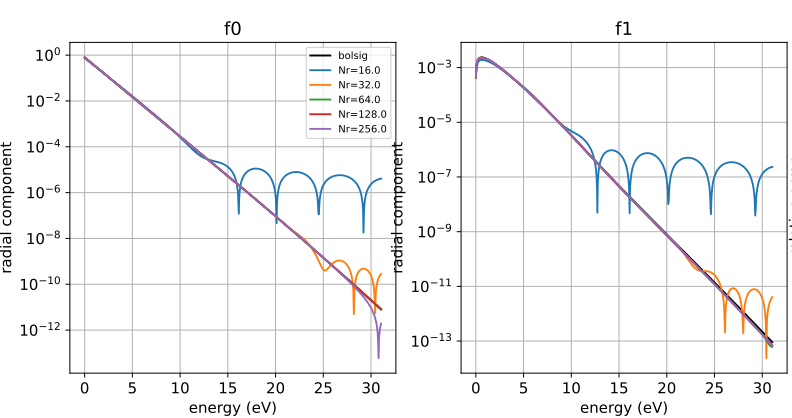
\includegraphics[width=0.48\textwidth]{1TD_ion_deg_1e-1.png}\\
% 			\end{tabular}}
% 	\end{minipage}
% 	\end{center}
% 	\begin{itemize}
% 		\item Beyond two-term approximation $E/N = 100Td \text{ and } n_e/N=1e-3$
% 	\end{itemize}
% 	\begin{center}
% 	\begin{minipage}{0.83\textwidth}
% 		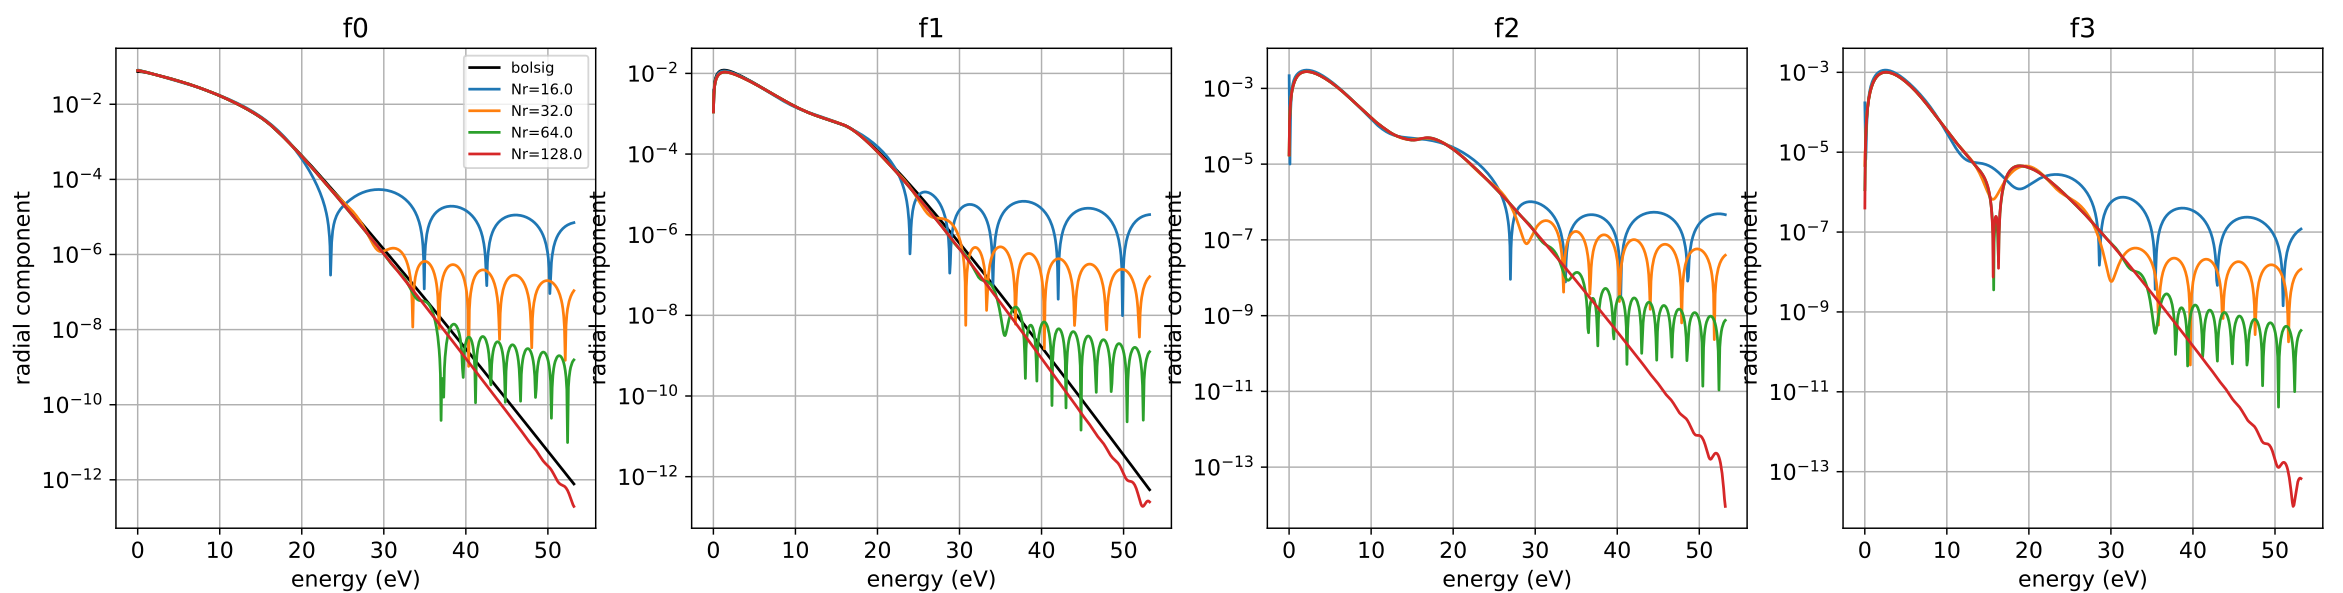
\includegraphics[width=\textwidth]{100Td_ion_deg1e-3.png}
% 	\end{minipage}
% 	\end{center}

% }



%----------------------------------------------------------------------------------------

\end{poster}

\end{document}
